\section{Experiments}

\begin{table*}[ht]
\centering
% \renewcommand{\arraystretch}{1.2}
% \setlength{\tabcolsep}{4pt}
\begin{tabular}{l|l|cccc|ccc|c}
\toprule
\multirow{2}{*}{\textbf{Model}} & \multirow{2}{*}{\textbf{Method}} & \multicolumn{4}{c|}{\textbf{LibriSpeech}} & \multicolumn{3}{c|}{\textbf{PPA}} &\multirow{2}{*}{\textbf{LLM\_dys}}\\
& & \textit{test-clean} & \textit{test-other} & \textit{dev-clean} & \textit{dev-other} & \textit{nfvppa} & \textit{lvppa} & \textit{svppa} & \\
\midrule
\multirow{3}{*}{\textbf{Wav2Vec2.0-L}} 
& CTC      & 16.16 & 21.04 & 15.41 & 20.50 & 41.04 & 36.63 & 15.78 & 14.52 \\
& CE-CTC   & 16.84 & 21.16 & 15.73 & 20.68 & 38.89 & 38.75 & 17.18 & 14.75 \\
& LCS-CTC\textit{(ours)}  & \textbf{16.09} & \textbf{20.94} & \textbf{15.10} & \textbf{19.70} & \textbf{38.14} & \textbf{32.04} & \textbf{15.01} & \textbf{13.89} \\
\midrule
\multirow{3}{*}{\textbf{HuBERT-L }} 
& CTC      & 15.00 & 18.16 & 14.12 & 17.18 & 32.70 & 18.34 & 13.32 & 12.13 \\
& CE-CTC   & 14.83 & 17.75 & 14.02 & 17.07 & 34.45 & 19.06 & 15.24 & 12.94 \\
& LCS-CTC\textit{(ours)}  & \textbf{14.75} & \textbf{17.35} & \textbf{11.78} & \textbf{16.72} & \textbf{32.02} & \textbf{17.71} & \textbf{13.30} & \textbf{11.85} \\
\midrule
\multirow{3}{*}{\textbf{WavLM-L}} 
& CTC      & 12.62 & 15.01 & 13.92 & 14.99 & 29.88 & 20.33 & 14.14 & 12.13 \\
& CE-CTC   & 12.31 & 14.73 & 12.83 & 14.90 & 30.34 & 22.15 & 15.05 & 11.30 \\
& LCS-CTC\textit{(ours)}  & \textbf{12.09} & \textbf{14.45} & \textbf{12.41} & \textbf{14.73} & \textbf{29.51} & \textbf{18.72} & \textbf{13.83} & \textbf{11.22} \\
\bottomrule
\end{tabular}
\caption{PER(\%) performance of three methods on LibriSpeech, PPA, and LLM\_dys dataset.}
\label{tab:per-results}
 \vspace{-5pt}
\end{table*}
\begin{table*}[ht]
\centering
\begin{tabular}{l|l|cccc|ccc|c}
\toprule
\multirow{2}{*}{\textbf{Model}} & \multirow{2}{*}{\textbf{Method}} & \multicolumn{4}{c|}{\textbf{Librispeech}} & \multicolumn{3}{c|}{\textbf{PPA}} & \multirow{2}{*}{\textbf{LLM\_dys}} \\
 & & \textit{test-clean} & \textit{test-other} & \textit{dev-clean} & \textit{dev-other} & \textit{nfvppa} & \textit{lvppa} & \textit{svppa} & \\
\midrule
\multirow{3}{*}{\textbf{WavLM-L}} 
 & CTC & 10.75 & 13.41 & 11.96 & 12.07 & 23.14 & 11.46 & 11.70 & 6.26 \\
 & CE-CTC & 10.73 & 13.41 & 11.70 & 12.14 & 23.55 & 13.05 & 12.94 & 5.71 \\
 & LCS-CTC\textit{(ours)} & \textbf{10.49} & \textbf{12.85} & \textbf{11.56} & \textbf{11.97} & \textbf{22.75} & \textbf{10.92} & \textbf{11.00} & \textbf{5.64} \\
\bottomrule
\end{tabular}
\caption{WPER(\%) performance of three methods on LibriSpeech, PPA, and LLM\_dys dataset.}
\label{tab:wper-results}
 \vspace{-5pt}
\end{table*}

\begin{table*}[ht]
\centering
% \renewcommand{\arraystretch}{1.3}
% \setlength{\tabcolsep}{6pt}
\begin{tabular}{c|c|cccc|c}
\toprule
\multirow{2}{*}{\textbf{Model}} & \multirow{2}{*}{\textbf{Method}} 
& \multicolumn{4}{c|}{\textbf{Librispeech}} & \multirow{2}{*}{\textbf{LLM\_dys}} \\
& & \textit{test-clean} & \textit{test-other} & \textit{dev-clean} & \textit{dev-other} & \\
\midrule
\multirow{2}{*}{\textbf{WavLM-L}} 
& CTC      & 146.6 & 113.5 & 115.8 & 131.3 & 95.1 \\
& LCS-CTC\textit{(ours)}  & \textbf{115.8} & \textbf{94.5} & \textbf{94.9} & \textbf{102.9} & \textbf{76.7} \\
\bottomrule
\end{tabular}
\caption{BL(ms) performance of different methods on LibriSpeech and LLM\_dys dataset.}
\label{tab:boundary-loss}
 \vspace{-5pt}
\end{table*}

\begin{table*}[ht]
\centering
% \renewcommand{\arraystretch}{1.3}
% \setlength{\tabcolsep}{6pt}
\begin{tabular}{c|c|cccc|c}
\toprule
\multirow{2}{*}{\textbf{Model}} & \multirow{2}{*}{\textbf{Method}} 
& \multicolumn{4}{c|}{\textbf{Librispeech}} & \multirow{2}{*}{\textbf{LLM\_dys}} \\
& & \textit{test-clean} & \textit{test-other} & \textit{dev-clean} & \textit{dev-other} & \\
\midrule
\multirow{2}{*}{\textbf{WavLM-L}} 
& CTC      & 22.4 & 14.8& 19.7 & 28.0 & 17.9 \\
& LCS-CTC\textit{(ours)}  &\textbf{16.0}  & \textbf{10.8} & \textbf{13.1} & \textbf{21.9} & \textbf{12.7} \\
\bottomrule
\end{tabular}
\caption{ARL performance of different methods on LibriSpeech and LLM\_dys dataset.}
\label{tab:arl-loss}
    \vspace{-10pt}
\end{table*}


\subsection{Datasets}
We use \textbf{VCTK}~\cite{yamagishi2019cstr-vctk} dataset which includes 109 native English speakers with accented speech to train our cost matrix learning model and phoneme recognition model, and we conduct experiments on three ASR datasets to evaluate our proposed LCS-CTC's performance: (1) \textbf{Librispeech}~\cite{7178964}, which contains 1000 hours of English speech, we use its \textit{dev} and \textit{test} subsets for evaluation. (2) \textbf{PPA
Speech}~\cite{gorno2011classification-ppa}, it is collected in collaboration with clinical experts and includes recordings from 38 participants diagnosed with
Primary Progressive Aphasia (PPA). Participants were asked to
read the ”grandfather passage,” resulting in approximately one
hour of speech in total. (3) \textbf{LLM\_dys}, as mentioned in~\cite{zhang2025analysisevaluationsyntheticdata}, We used a large language model (claude-3-5-sonnet-20241022~\cite{anthropic2024claude}) to create a synthetic speech dataset. Given clean text and its CMU/IPA sequences, the model was prompted to insert dysfluencies naturally. This produced dysfluent IPA sequences for VITS-based speech synthesis~\cite{kim2021conditionalvariationalautoencoderadversarial}, as well as CMU sequences labeled with dysfluencies for evaluation. 
\subsection{Implementation details}
In our main experiments, we split the VCTK dataset into four partitions with a ratio of 3:1:5:1. Specifically, 30\% of the data is used for training the cost matrix learning model. These samples are annotated with MFA and manual refinement, mentioned in Section~\ref{sec:lcs-align}. An additional 10\% is held out as the validation set for this stage.

For training the phoneme recognition model based on our proposed LCS-CTC, we use 50\% of the data for training and 10\% for validation. All experiments are conducted on an NVIDIA A6000 GPU. We use a learning rate of $1\text{e}{-5}$ and a batch size of 1 for all training stages. No weight decay is applied during optimization.

\subsection{Evaluation Metrics}
\subsubsection{Phoneme Error Rate (PER)}
Phoneme Error Rate is a common metric for evaluating phoneme-level recognition performance. It is defined as the Levenshtein distance between the predicted and reference phoneme sequences, normalized by the length of the reference. The metric accounts for substitution, insertion, and deletion errors, and reflects the overall transcription accuracy at the phonetic level.
\subsubsection{Weighted Phonetic Error Rate (WPER)}Unlike PER which assumes all phonemes are equally distant, WPER takes phonetic variation into account by incorporating phoneme similarity. This addresses the shortcomings of traditional error metrics and offers a more accurate evaluation of recognition performance. Refer to~\cite{guo2025dysfluentwfstframeworkzeroshot}, we define WPER as
\[
\text{WPER} = \frac{\sum_{(p_t,p_s)} (1 - s(p_t,p_s)) + D + I}{N}
\]

where \( p_t, p_s \) denote target and substitute phonemes, \( s \) is their similarity score defined in \ref{sec:lcs-align}, 
and \( N \) is the reference phoneme sequence length. \( D \) and \( I \) represent deletion 
and insertion errors respectively. For substitutions, phoneme similarity is evaluated first,
followed by error penalties.
\subsubsection{Boundary Loss (BL)}
Boundary Loss (BL) quantifies the alignment quality between predicted and ground-truth phoneme boundaries. Specifically, it is computed as the average absolute deviation between the predicted and reference onset/offset times of each phoneme. A lower BL reflects more accurate temporal alignment.
\subsubsection{Articulatory Reconstruction Loss (ARL)}
To assess phoneme-level articulatory consistency, we introduce ARL. It measures the L2 distance between articulatory embeddings reconstructed from predicted phonemes and those extracted from the original audio using an acoustic-to-articulatory inversion (AAI) model~\cite{Cho_2024}. Lower ARL indicates better articulatory plausibility of the recognition output.

\subsection{Results and Discussion}


\begin{figure*}[t]
    \centering
    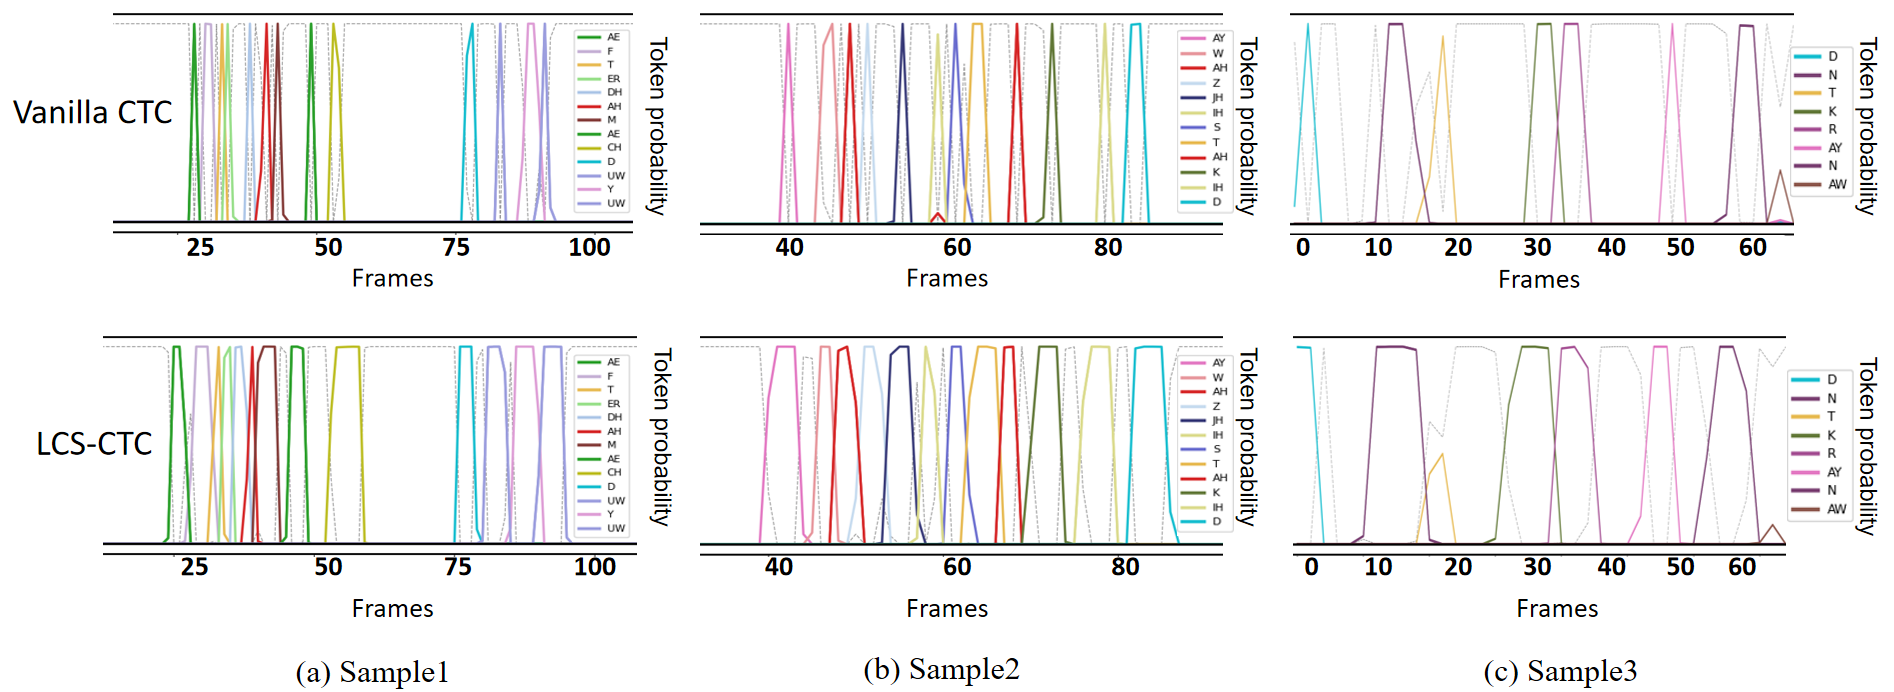
\includegraphics[width=15.0cm]{figure/res.png}
    \caption{Visualization of token emission probabilities for vanilla CTC and our proposed LCS-CTC on three randomly selected samples from the LibriSpeech and PPA. The gray dashed lines indicate the blank token. Compared to vanilla CTC, LCS-CTC produces smoother and more distributed token activations, characterized by more consistent repetitions of non-blank tokens.}
    \label{fig:emission}
     \vspace{-10pt}
\end{figure*}

Table~\ref{tab:per-results} presents the PER of different training methods, including vanilla CTC and our proposed LCS-CTC—applied to three common speech encoders: Wav2Vec2.0~\cite{baevski2020wav2vec20frameworkselfsupervised}, HuBERT~\cite{hsu2021hubertselfsupervisedspeechrepresentation}, and WavLM~\cite{Chen_2022}. Across all models and datasets, LCS-CTC outperforms vanilla CTC on both clean (e.g., test-clean, dev-clean) and challenging conditions (e.g., test-other, lvppa, LLM\_dys), demonstrating strong generalization.

We also compare with CE-CTC, a variant that combines CTC with frame-level cross-entropy loss derived from ground-truth alignments. While CE-CTC introduces additional frame-level supervision, it does not consistently outperform vanilla CTC, especially on more challenging datasets such as PPA and LLM\_dys. This suggests that relying on full-frame labels does not always lead to better generalization, and may even introduce noise under dysfluent or noisy speech conditions. In contrast, LCS-CTC achieves competitive or superior performance without relying on frame-level labels at training time, making it more practical and scalable.

Furthermore, we report WPER in Table~\ref{tab:wper-results} using the best-performing encoder WavLM. LCS-CTC again shows the best performance on all subsets. These results confirm that our method leads to more accurate and robust phoneme recognition across various speech conditions.


We use Boundary Loss (BL) to measure alignment quality. As shown in Table~\ref{tab:boundary-loss}, LCS-CTC significantly reduces BL compared to vanilla CTC, indicating more accurate and temporally consistent alignments. This is further supported by the emission visualizations in Fig.~\ref{fig:emission}, where LCS-CTC produces smoother and less peaky token distributions. Such smoother emission behavior enhances generalization and likely contributes to the improved recognition performance observed earlier. Moreover, our model can also serve as a text-free phoneme-level aligner. The results in Table~\ref{tab:arl-loss} demonstrate that LCS-CTC yields consistently lower articulatory reconstruction loss compared to vanilla CTC. This suggests that the phoneme sequences predicted by LCS-CTC better preserve articulatory smoothness and continuity, leading to embeddings that more closely match the natural trajectories derived from the speech signal.

\subsection{Ablation experiments}\label{abl}
\vspace{-5pt}
\begin{figure}[ht]
  \centering
  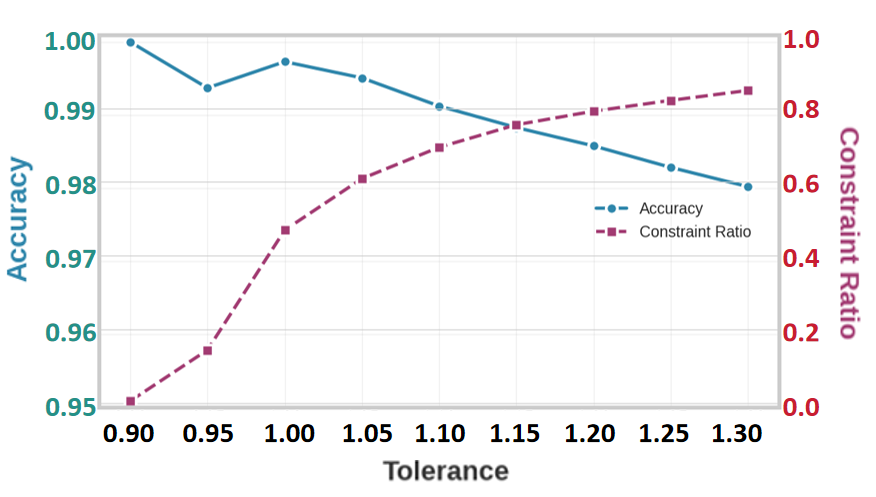
\includegraphics[width=0.9\columnwidth]{figure/tol.png}
  \caption{Effect of \textit{tol} on alignment accuracy and constrained region ratio.}
  \label{fig:tol}
  \vspace{-5pt}
\end{figure}
We perform an ablation study on the tolerance parameter $\mathit{tol}$ in the LCS alignment algorithm, which controls the threshold for accepting frame-phoneme matches based on predicted cost and phoneme similarity. Smaller values of $\mathit{tol}$ impose stricter alignment conditions, leading to higher alignment precision but fewer constrained regions. This may reduce the effectiveness of the frame-level supervision in our LCS-CTC. In contrast, larger $\mathit{tol}$ values include more frames but risk introducing noisy or imprecise alignments, which can weaken training. We evaluate values in the range $\{0.9-1.3\}$ and observe that $\mathit{tol} = 1.0$ provides the best balance between alignment accuracy and coverage, and is thus adopted in all main experiments.
